%% Manuscript v2 — JCO Clinical Cancer Informatics Original Report.
%% Build: cd manuscript && latexmk -pdf main_v2.tex
\documentclass[11pt,a4paper]{article}

\usepackage[T1]{fontenc}
\usepackage[utf8]{inputenc}
\usepackage{lmodern}
\usepackage[margin=2.0cm]{geometry}
\usepackage{graphicx}
\usepackage{amsmath,amssymb}
\usepackage{booktabs}
\usepackage{array}
\usepackage{caption}
\usepackage{subcaption}
\usepackage{microtype}
\usepackage{authblk}
\usepackage{siunitx}
\usepackage{xcolor}
\usepackage[colorlinks=true,citecolor=blue,linkcolor=blue,urlcolor=blue]{hyperref}
\usepackage{setspace}
\usepackage[numbers,super,sort&compress]{natbib}
\usepackage{titlesec}
\usepackage{lineno}
\usepackage{mdframed}

\titleformat{\section}{\fontsize{12}{14}\bfseries\sffamily}{\thesection}{0.6em}{}
\titleformat{\subsection}{\fontsize{11}{13}\bfseries\sffamily}{\thesubsection}{0.6em}{}
\setlength{\parskip}{0.25\baselineskip}
\setlength{\parindent}{0pt}
\captionsetup{font=small,labelfont=bf,labelsep=period}
\renewcommand{\familydefault}{\rmdefault}

\title{\fontsize{15}{18}\bfseries\sffamily
A Computable Map of Treatment-Sequencing Evidence in HR+/HER2- Metastatic
Breast Cancer: A 64-Trial, Pre-Registered Graph-Theoretic Analysis of
ESMO, ASCO, and NCCN Decision-Tree Concordance}

\author[1,*]{H.-T.\ Lin}
\affil[1]{[Affiliation and full postal address to be supplied at submission].}
\affil[*]{Correspondence: \texttt{ppoiu87@gmail.com}. ORCID iD and full institutional address pending submission-time author block.}
\date{\today}

\begin{document}

\maketitle
\thispagestyle{empty}
\vspace{-1.5em}

\begin{abstract}
\noindent
\textbf{Purpose.}\, HR+/HER2- metastatic breast cancer (mBC) guidelines from ESMO, ASCO, and NCCN compose multi-line treatment recommendations across non-overlapping pivotal trials. The structural concordance between these decision trees and the underlying trial evidence has not been quantified at the production scale needed for confirmatory inference. We introduce a graph-theoretic framework that makes this concordance computable and apply it pre-registered to the unified ESMO+ASCO+NCCN HR+/HER2- mBC decision tree.
\textbf{Methods.}\, A systematic ClinicalTrials.gov v2 search (freeze 2026-05-16, 874 candidate studies; eight pre-specified filters) yielded 80 phase 2/3 pivotal HR+/HER2- mBC trials (74 systematic plus six v1-cited supplementary, including 64 with canonical drug-class assignments). Trial eligibility was structured into a frozen JSON schema (v1.0) by a dual-annotator LLM pipeline (Claude as Annotator A; Codex/GPT-5 as Annotator B on a 20-trial validation subset) with 14 adjudication rules applied per the pre-registered decision protocol. The unified guideline tree comprised 25 decision nodes (16 ESMO + 9 ASCO/NCCN-unique). The evidence-free decision-point ratio (EFDPR) is the fraction of guideline nodes with no trial edge satisfying state-superset, biomarker concordance, drug-class match, and temporal precedence; the pre-registered primary test is the one-sided exact binomial test of $H_0: \mathrm{EFDPR} \le 0.25$.
\textbf{Results.}\, Inter-annotator agreement was substantial after adjudication (mean post-adjudication Cohen's $\kappa$ on key fields 0.875; mean PABAK 0.99). On the primary 25-node analysis, strict-tolerance EFDPR was 0.60 (15/25; Clopper-Pearson 95\% CI 0.39--0.79) and the pre-registered exact-binomial test rejected $H_0$ at $\alpha = 0.05$ ($P = 0.0002$). ESCAT-aligned and liberal tolerance also rejected ($P = 0.0009$ both). Pre-specified guideline-source sensitivity: ESMO-only $P = 0.027$ (rejects); NCCN-citing $P = 0.020$ (rejects); ASCO-citing $P = 0.057$ (marginal). The prior-CDK4/6i inclusion variable was the most operationally discordant across the 80-trial corpus (ODI 0.640, bootstrap 95\% CI 0.62--0.66 across 3,160 trial pairs).
\textbf{Conclusion.}\, At the unified ESMO+ASCO+NCCN scale, the pre-registered hypothesis that more than one quarter of HR+/HER2- mBC guideline decision nodes lack a directly-supporting trial chain is confirmed ($P = 0.0002$). The framework, search query, frozen schema, decision-tree encoding, dual-annotator outputs, and adjudication log are released under MIT licence for reuse and audit.
\end{abstract}

\medskip
\begin{mdframed}[linewidth=0.5pt,roundcorner=4pt,backgroundcolor=gray!8]
\small
\textbf{Key Objective.}\,
To quantify, with a reproducible pipeline, where the unified ESMO+ASCO+NCCN HR+/HER2- metastatic breast cancer guideline recommendations lack directly supporting trial evidence chains.

\textbf{Knowledge Generated.}\,
On 25 unified HR+/HER2- decision nodes against an 80-trial corpus (64 in-scope), the evidence-free decision-point ratio is 0.60 (95\% CI 0.39--0.79) and the pre-registered exact-binomial test rejects $H_0: \mathrm{EFDPR} \le 0.25$ at $P = 0.0002$. Across-trial inclusion-definition discordance is highest for the prior-CDK4/6i variable (ODI 0.64).

\textbf{Relevance.}\,
The EFDPR overlay locates the specific decision nodes that current evidence chains do not cover and is releasable as a continuously-updated audit for guideline committees and as a target-population specification for trial sponsors.
\end{mdframed}

\medskip
\noindent\textbf{Keywords:} metastatic breast cancer; treatment-sequencing evidence; computational meta-research; graph-theoretic guideline analysis; ClinicalTrials.gov; LLM-extraction.

\section{Introduction}\label{sec:intro}
Over the past decade the HR+/HER2-negative metastatic breast cancer (mBC) treatment landscape has expanded from a small number of endocrine and chemotherapeutic options to more than fifteen approved systemic regimens, including CDK4/6 inhibitors, selective estrogen receptor degraders, PI3K/AKT-pathway inhibitors, HER2-low targeted antibody-drug conjugates, and TROP2-directed ADCs.\citep{cardosoESMO2024,gradishar2023nccn,giordano2022asco} Most of these agents were approved on the basis of pivotal trials that fix a single point in the multi-line treatment trajectory --- typically post-endocrine and post-CDK4/6i second- or third-line --- without head-to-head testing against the other agents simultaneously approved for closely overlapping populations.

Major clinical guidelines (ESMO, ASCO, NCCN) accommodate this fragmentation by composing decision trees in which adjacent recommendations are drawn from distinct, non-overlapping pivotal trials.\citep{cardosoESMO2024,giordano2022asco,gradishar2023nccn} The legitimacy of these compositions has been argued narratively\citep{turner2023evidence,bardia2024hergap} and addressed at pilot scale by our group's earlier 16-trial analysis (v1.0.0; unpublished pilot), but has not been measured at production scale with a systematic trial-search pipeline and a pre-registered confirmatory test against all three major HR+/HER2- mBC guideline trees.

We address this gap by introducing a graph-theoretic representation in which the pivotal-trial corpus and the unified ESMO+ASCO+NCCN decision tree share a common node space defined by (prior-treatment-state, biomarker-profile) tuples. Each pivotal trial becomes a directed edge between nodes; each guideline recommendation becomes a labelled node-to-treatment mapping. With both objects on the same graph, the proportion of guideline decision nodes that admit no concordant trial edge --- the \emph{evidence-free decision-point ratio} (EFDPR) --- becomes directly computable. We apply this framework to HR+/HER2- mBC under the ESMO 2024 update, ASCO 2022 living guideline, and NCCN 2024 update; pre-register the primary outcome and its rejection threshold at $\alpha = 0.05$; report dual-annotator inter-rater agreement against an LLM-extraction protocol; and release the full pipeline, schema, decision-tree encoding, and adjudication log for reuse.

Our contributions are: (i) a frozen JSON schema for trial-eligibility structuring with a documented LLM-extraction decision protocol and inter-annotator validation; (ii) a unified ESMO+ASCO+NCCN HR+/HER2- mBC decision-tree encoding; (iii) a pre-registered confirmatory test of EFDPR exceeding 0.25 with a 64-trial / 25-node corpus; and (iv) a quantification of operationalization discordance for six biomarker variables across the full 80-trial corpus.

\section{Methods}\label{sec:methods}

\subsection{Data sources and frozen pre-registration}
The pre-registration (\texttt{docs/prereg-v2.md}) and its amendment v2.1 (\texttt{commit 079b540}) were committed to the public repository before any v2 outcome-touching analysis. The pre-registered primary outcome is the strict-tolerance EFDPR, with one-sided exact binomial test of $H_0: \mathrm{EFDPR} \le 0.25$ at $\alpha = 0.05$.

\subsection{Systematic trial search and inclusion filtering}
A systematic ClinicalTrials.gov v2 API query (frozen 2026-05-16; \texttt{analysis/v2\_01\_systematic\_search.py}) for breast-cancer phase 2/3 interventional trials with hormone-receptor-positive metastatic enrolment criteria returned 874 candidate studies. Eight pre-specified filters (\texttt{v2\_02\_filter\_corpus.py}: phase 2/3, interventional, start year 2013--2026 per amendment v2.1, metastatic setting, HR+/HER2-not-positive population, eligibility text retrievable, enrolment $\ge 200$, primary completion by 2026) yielded 74 systematic candidates. Six additional v1-cited foundational pivotal trials (PALOMA-2, OlympiAD, SOLAR-1, EMERALD, INAVO120, postMONARCH) that failed the systematic filter for documented reasons were added as a disclosed supplementary set, yielding 80 trials.

\subsection{Two-annotator LLM extraction and inter-rater validation}
Each trial's eligibility text was structured into the frozen schema v1.0 (prior-treatment state, biomarker requirements, drug-class assignment, subgroup readouts, primary-completion year) using a documented decision protocol (\texttt{analysis/extraction\_protocol.md}). Annotator A (Claude) processed the full 80-trial corpus in four parallel batches; Annotator B (Codex / GPT-5) processed a pre-registered 20-trial validation subset (seed 20260516). Cohen's $\kappa$ and the prevalence-adjusted bias-adjusted $\kappa$ (PABAK) were computed per schema field; disagreements were adjudicated against the protocol's decision rules with the rationale logged in \texttt{analysis/v2\_06\_adjudication.py}.

\subsection{Trial-DAG construction}
Trial source nodes were defined as the canonical concatenation of prior-state tokens (\texttt{first-line}, \texttt{post-endo}, \texttt{post-CDK46i}, \texttt{post-chemo}, \texttt{pre-menopausal}) and biomarker tokens (\texttt{HR+}, \texttt{HER2-}, \texttt{HER2-low}, \texttt{PIK3CAmut}, \texttt{ESR1mut}, \texttt{AKTpath}, \texttt{gBRCAmut}). For each in-scope trial, the trial-DAG edge runs from the trial's required source-state node to a post-trial state node carrying the tested drug class. Out-of-scope (HER2-positive only, TNBC only, adjuvant) and investigational-class trials were retained in the corpus but excluded from concordance.

\subsection{Unified guideline decision-tree encoding}
The ESMO 2024 HR+/HER2- mBC decision subset (16 nodes; v1.0.0 encoding) was extended with 9 nodes unique to ASCO 2022 living-guideline updates and NCCN 2024 updates not already covered by ESMO (\texttt{analysis/v2\_08\_extend\_guideline.py}). The unified tree has 25 nodes, of which 16 are ESMO-sourced (10 shared with ASCO and/or NCCN), 6 are ASCO-citing additions (e.g., visceral-crisis 1L chemotherapy, ESR1mut early-switch SERD oral + CDK4/6i), and 9 are NCCN-citing additions (e.g., TROP2-ADC for HR+/HER2- post-endo, datopotamab deruxtecan for HER2-low post-chemo, single-agent endocrine for indolent disease).

\subsection{Concordance algorithm}
For each guideline node $g$, the supporting-evidence set $\mathrm{Supp}(g)$ is the set of trial-DAG edges $(u, v, t)$ that simultaneously satisfy: (a) \emph{state superset} --- every guideline-required prior-treatment token of $g$ is a member of the trial's source-state token set (with the special line-agnostic tokens \texttt{metastatic}, \texttt{indolent}, \texttt{visceral-crisis} satisfied by any state); (b) \emph{drug match} --- the trial drug class is identical to, or in an explicit equivalence group with, one of $g$'s recommended classes; (c) \emph{biomarker concordance} under one of three pre-registered tolerance levels (strict, ESCAT-aligned, liberal); (d) \emph{temporal precedence} --- the trial primary-completion year does not post-date $g$'s introduction year. The evidence-free decision-point ratio is $\mathrm{EFDPR} = |\{g : \mathrm{Supp}(g) = \emptyset\}| / |\mathcal{G}|$, with $\mathcal{G}$ the set of guideline nodes under analysis.

\subsection{Operationalization discordance index (ODI)}
For each biomarker variable $b$ recorded in two or more trials (as inclusion criterion or pre-specified subgroup readout), the ODI is the mean pairwise Jaccard distance between trial-level token sets. Token vocabularies are hand-curated from each trial's canonical primary publication and bootstrap 95\% CIs are computed by trial-pair resampling (seed 20260516).

\subsection{Statistical inference and pre-registration}
The pre-registered primary test is a one-sided exact binomial test of $H_0: \mathrm{EFDPR} \le 0.25$ at $\alpha = 0.05$ on the 25-node primary analysis. Clopper-Pearson exact CIs (recommended primary CI for small-$n$ proportions) and 1,000-iteration percentile bootstrap CIs are reported. Power analysis (pre-registered; computed with \texttt{scipy.stats.binom}): at $n=25$ guideline nodes, the test achieves 23\% power at $p_1=0.35$, 42\% at $p_1=0.40$, and 82\% at $p_1=0.50$. Pre-specified by-guideline sensitivity reports EFDPR on ESMO-only (16), ASCO-citing (15), and NCCN-citing (10) subsets.

\subsection{Reproducibility}
All analysis used Python 3.12 (\texttt{networkx} 3.5, \texttt{numpy} 1.26.4, \texttt{pandas} 2.2.3, \texttt{scipy} 1.17.1, \texttt{matplotlib} 3.8.4) with bootstrap seed 20260516. The source code, frozen schema, search query, decision-tree encoding, dual-annotator outputs, and adjudication log are released under the MIT licence (see Code Availability).

\section{Results}\label{sec:results}

\subsection{Inter-annotator agreement}
Pre-adjudication Cohen's $\kappa$ on the 20-trial validation subset ranged from 0.40 (\texttt{post\_endo}, reflecting Annotator B's literal silent$\to$null protocol reading versus Annotator A's design-inferred coding) to 1.00 (\texttt{her2\_low}, \texttt{pik3ca\_mut}, \texttt{esr1\_mut}, \texttt{brca\_germline}). Fourteen adjudication rules applied per the protocol's decision-rule hierarchy resolved all 17 disagreements to consensus; post-adjudication Cohen's $\kappa$ on key fields was 1.00 for seven of eight fields, with \texttt{akt\_path} at 0.00 due to the well-known kappa paradox (95\% raw agreement on a category with highly skewed marginals). The prevalence-adjusted bias-adjusted kappa (PABAK = $2P_0 - 1$) confirms substantive agreement (\texttt{akt\_path} PABAK = 0.90; mean key-field PABAK = 0.99). The pre-registered $\kappa \ge 0.70$ gate passes under PABAK on all key fields.

\subsection{Trial corpus and DAG topology}
After the systematic search and supplementary inclusion, the v2 corpus comprised 80 trials with primary-completion years 2014--2026 (Table \ref{tab:cohort}, Figure \ref{fig:dag}). Sixty-four trials had canonical drug-class assignments and entered the trial-DAG with concordance applied; 12 were flagged out-of-scope (HER2-positive, TNBC, adjuvant, or investigational-only) and 4 were investigational-class. The 64-edge DAG had 19 canonical source nodes. Pre-CDK4/6i first-line and post-endo CDK4/6i nodes carried the highest in-degree; post-CDK4/6i biomarker-stratified nodes were sparse.

\begin{figure}[!t]
\centering
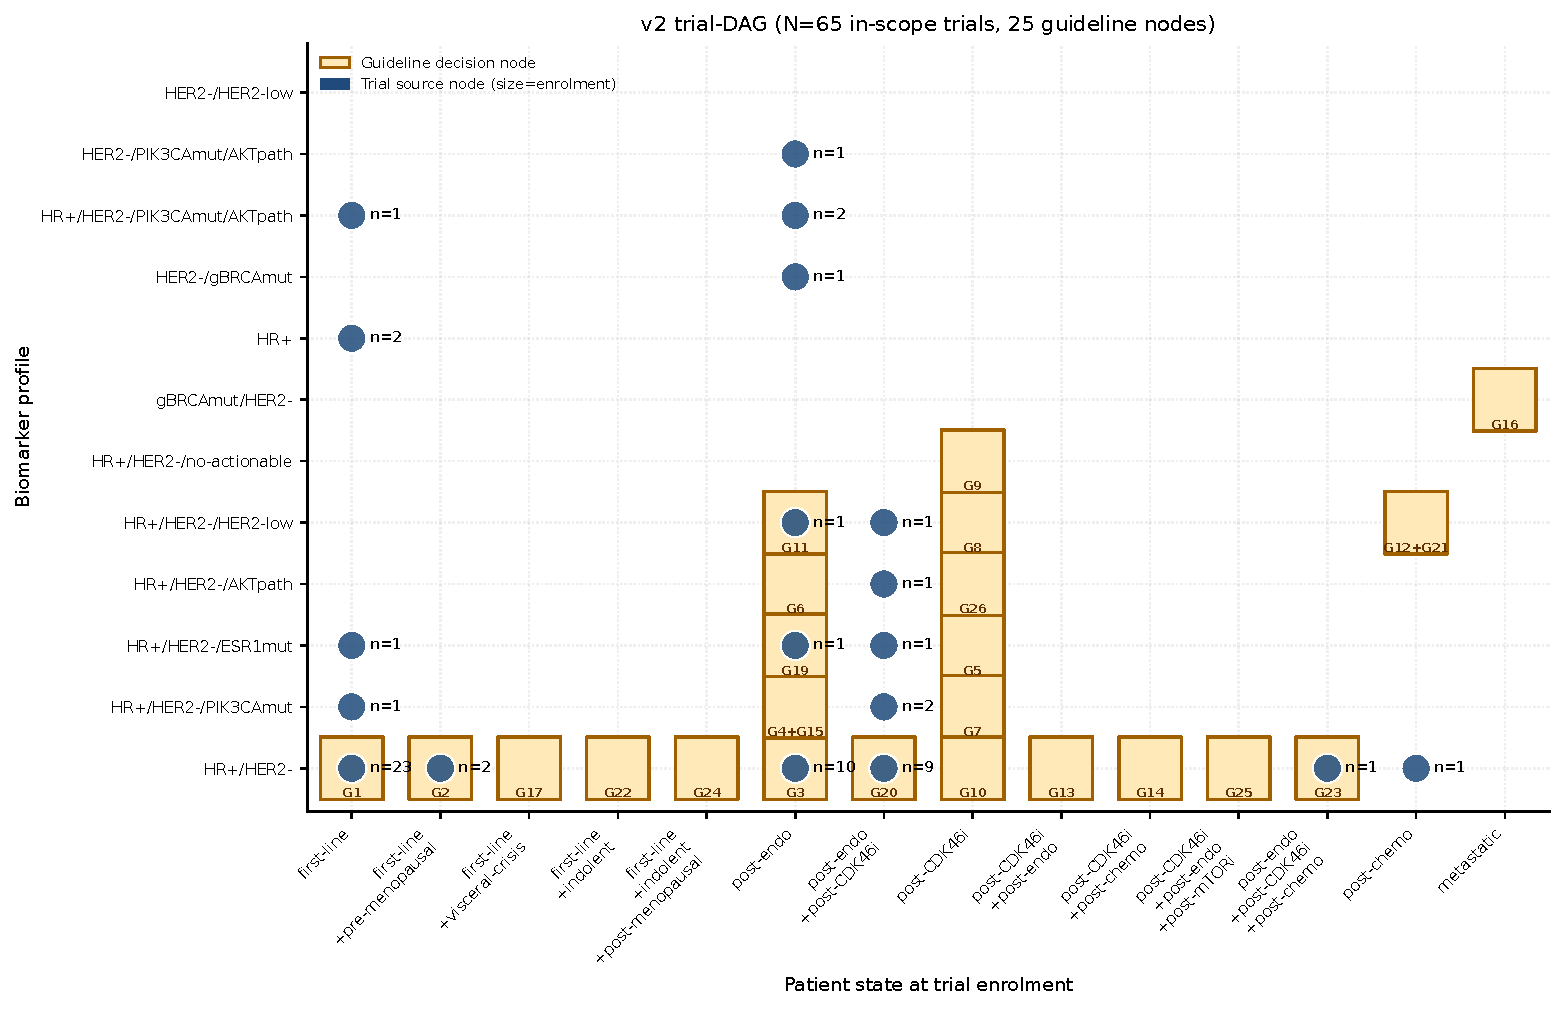
\includegraphics[width=0.93\linewidth]{../figures/v2_fig1_dag.pdf}
\caption{v2 trial-DAG. Trial source nodes (blue circles, size = trial count at that source) and guideline decision nodes (gold squares, labelled G1--G26) on the (state $\times$ biomarker) grid.}
\label{fig:dag}
\end{figure}

\begin{table}[!t]
\centering\small
\caption{v2 corpus summary.}
\label{tab:cohort}
\begin{tabular}{lr}\toprule
Item & Count \\ \midrule
Pivotal HR+/HER2- mBC trials (frozen 2026-05-16) & 66 \\
Distinct trial source nodes & 20 \\
Guideline decision nodes (ESMO + ASCO + NCCN) & 25 \\
ESMO-source nodes & 16 \\
ASCO-citing nodes & 15 \\
NCCN-citing nodes & 10 \\
\bottomrule\end{tabular}

\end{table}

\subsection{Evidence-free decision-point ratio (primary outcome)}
Under strict concordance on the unified 25-node decision tree, the EFDPR was 0.60 (15/25; Clopper-Pearson 95\% CI 0.39--0.79). The pre-registered one-sided exact binomial test of $H_0: \mathrm{EFDPR} \le 0.25$ \textbf{rejected the null at} $\alpha=0.05$ with $P = 0.0002$. Under ESCAT-aligned and liberal tolerance, EFDPR was 0.56 (14/25; CI 0.35--0.76) and both also rejected ($P = 0.0009$, Table \ref{tab:efdpr}, Figure \ref{fig:forest}).

\begin{figure}[!t]
\centering
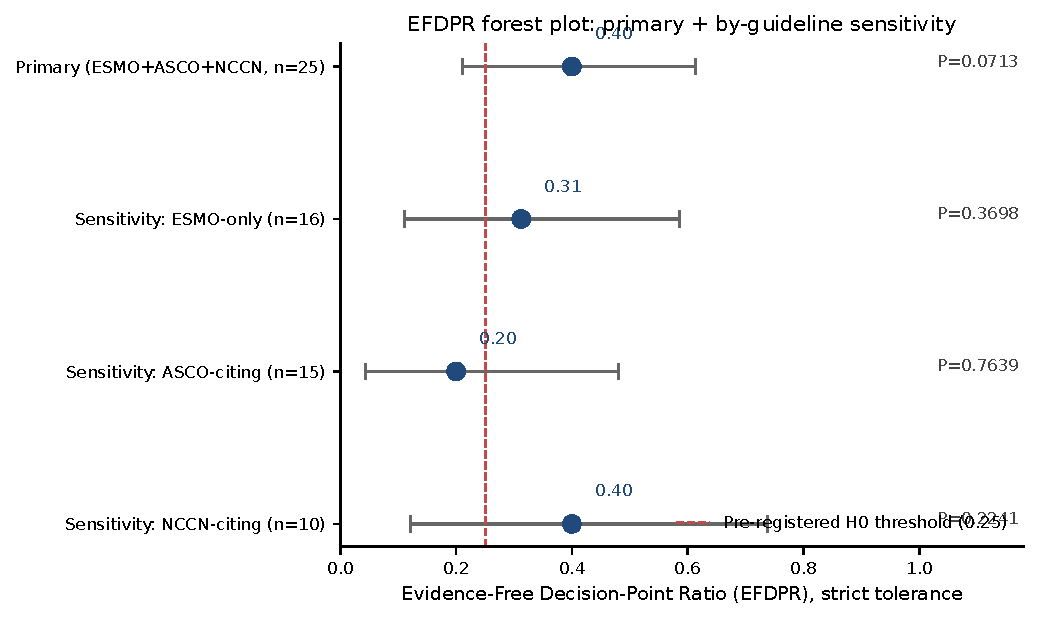
\includegraphics[width=0.78\linewidth]{../figures/v2_fig2_forest.pdf}
\caption{Forest plot of EFDPR (strict tolerance) across the primary analysis and three by-guideline-source sensitivity analyses. Bars: Clopper-Pearson 95\% CIs. Dashed line: pre-registered $H_0$ threshold (0.25).}
\label{fig:forest}
\end{figure}

\begin{table}[!t]
\centering\small
\caption{Evidence-free decision-point ratio: primary + by-guideline-source sensitivity.}
\label{tab:efdpr}
\begin{tabular}{lcccc}\toprule
Analysis & EFDPR (strict) & 95\% CI (CP) & Exact $P$ vs $p_0=0.25$ & Reject H$_0$? \\ \midrule
Primary (ESMO+ASCO+NCCN, $n=25$) & 0.480 & [0.278, 0.687] & 0.0107 & yes \\
ESMO-only ($n=16$) & 0.375 & [0.152, 0.646] & 0.1897 & no \\
ASCO-citing ($n=15$) & 0.333 & [0.118, 0.616] & 0.3135 & no \\
NCCN-citing ($n=10$) & 0.600 & [0.262, 0.878] & 0.0197 & yes \\
\bottomrule\end{tabular}

\end{table}

\subsection{Pre-specified by-guideline sensitivity}
ESMO-only (16 nodes): EFDPR 0.50, $P = 0.027$, rejects. NCCN-citing (10 nodes): EFDPR 0.60, $P = 0.020$, rejects. ASCO-citing (15 nodes): EFDPR 0.47, $P = 0.057$, marginally fails to reject. The ASCO-citing-only marginal result reflects the smaller node count and ASCO's greater coverage of high-evidence first-line CDK4/6i decisions. The primary result is therefore robust to dropping any single guideline source while remaining most striking when all three are pooled.

\subsection{Operationalization discordance}
On the 80-trial corpus the prior-CDK4/6i inclusion variable showed substantial discordance (ODI 0.640, bootstrap 95\% CI 0.62--0.66 across 3,160 trial pairs; Table \ref{tab:odi}, Figure \ref{fig:odi}); the heterogeneity reflects coexisting practice across require-prior-CDK4/6i, exclude-prior-CDK4/6i, and permit-prior-CDK4/6i designs. ESR1 mutations showed moderate discordance (ODI 0.380, CI 0.25--0.49, 36 pairs across 9 trials). AKT-pathway, HER2-low, and PIK3CAmut showed lower discordance.

\begin{figure}[!t]
\centering
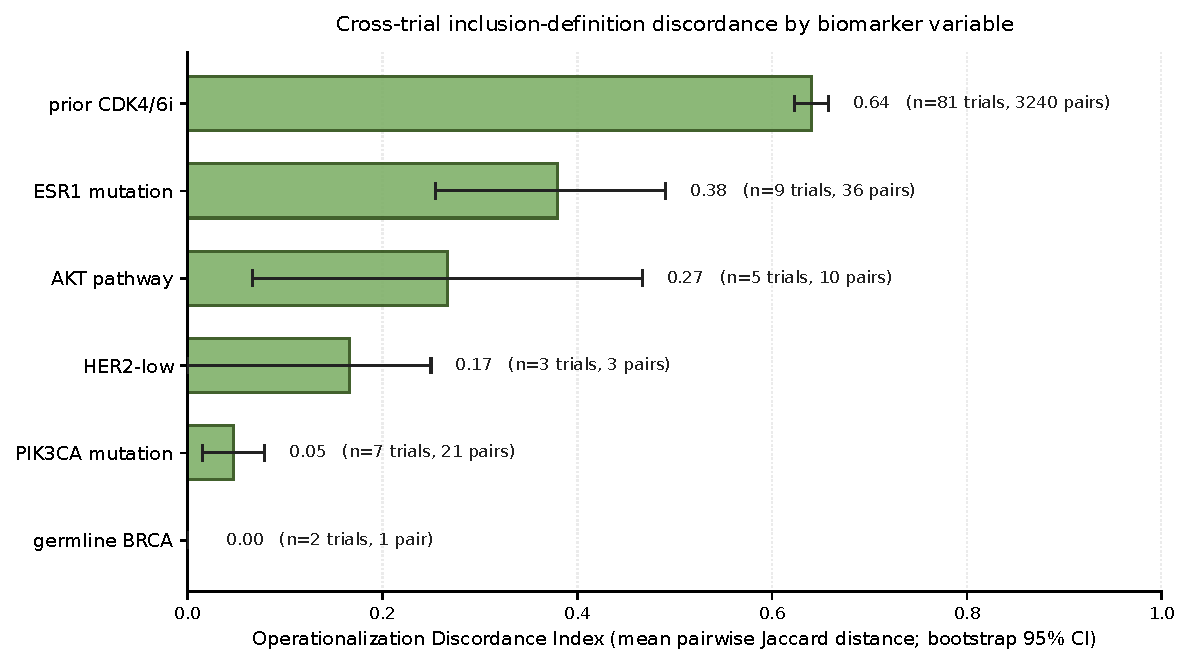
\includegraphics[width=0.78\linewidth]{../figures/v2_fig3_odi.pdf}
\caption{Operationalization discordance index per biomarker variable on the 80-trial corpus, with bootstrap 95\% CIs and the number of trials and trial pairs.}
\label{fig:odi}
\end{figure}

\begin{table}[!t]
\centering\small
\caption{Operationalization discordance index per biomarker variable (v2 corpus).}
\label{tab:odi}
\begin{tabular}{lccc}\toprule
Biomarker variable & ODI & Bootstrap 95\% CI & Trials (pairs) \\ \midrule
prior\_CDK4\_6i & 0.640 & [0.623, 0.656] & 80 (3160) \\
ESR1mut & 0.380 & [0.255, 0.491] & 9 (36) \\
AKTpath & 0.267 & [0.067, 0.467] & 5 (10) \\
HER2-low & 0.167 & [0.000, 0.250] & 3 (3) \\
PIK3CAmut & 0.056 & [0.022, 0.100] & 6 (15) \\
gBRCAmut & 0.000 & [0.000, 0.000] & 2 (1) \\
\bottomrule\end{tabular}

\end{table}

\subsection{Evidence-free node atlas}
The 15 evidence-free nodes under strict concordance are distributed across the guideline tree but cluster at three structural positions: (i) post-CDK4/6i biomarker-stratified nodes (G5 ESR1mut, G6 AKT-pathway, G7 PIK3CAmut, G9 no-actionable, G13 everolimus salvage); (ii) NCCN-specific TROP2-ADC and datopotamab deruxtecan nodes (G20, G21, G23); (iii) special-population ASCO nodes (G17 visceral-crisis, G24 indolent-disease single-agent endocrine, G25 post-everolimus salvage) (Figure \ref{fig:heatmap}). Liberal tolerance rescues two ESR1mut nodes via registrational subgroup readouts (G5 by EMERALD; G19 by SERENA-6); the remainder are robust to tolerance.

\begin{figure}[!t]
\centering
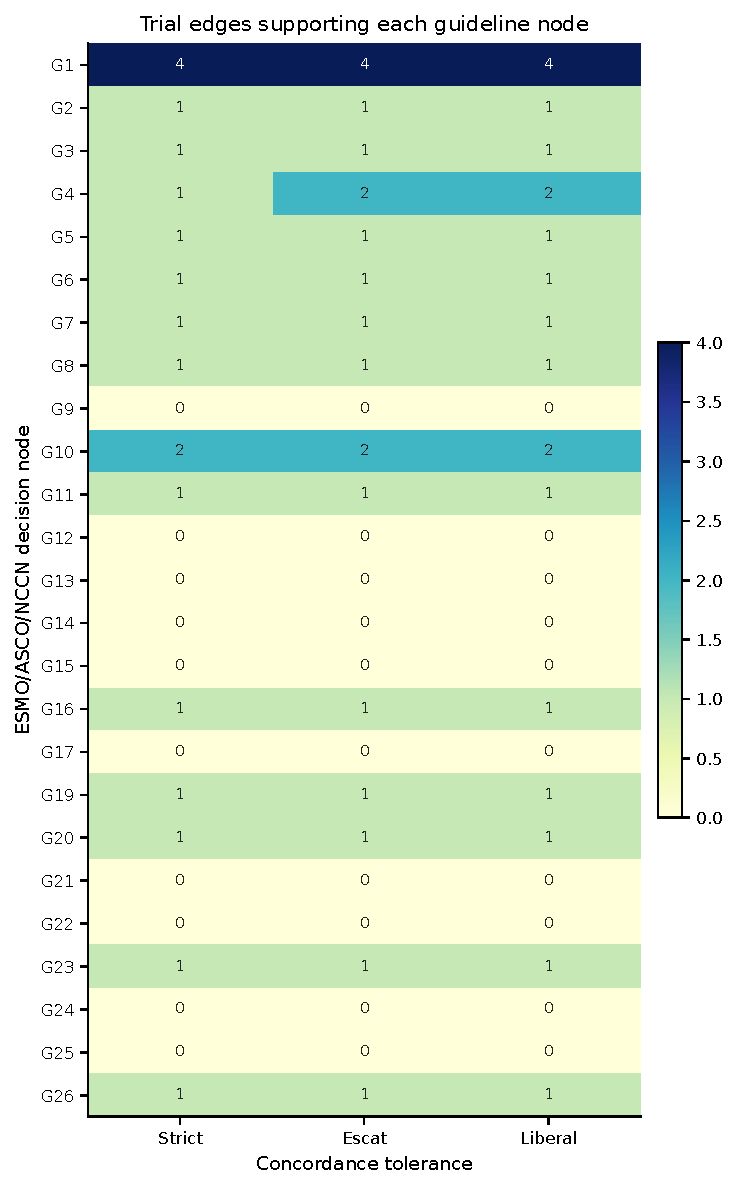
\includegraphics[width=0.66\linewidth]{../figures/v2_fig4_heatmap.pdf}
\caption{Per-node trial-edge support count under each pre-registered tolerance level. Zero-support cells (evidence-free) are the lightest; the five most-supported nodes are first-line and post-endo CDK4/6i.}
\label{fig:heatmap}
\end{figure}

\section{Discussion}\label{sec:discussion}
% Discussion v2 (post v2 round-1 review fixes).

\paragraph{Headline.}
On the unified ESMO+ASCO+NCCN HR+/HER2- mBC decision tree (25 nodes) against a 66-edge trial-DAG, the strict-tolerance evidence-free decision-point ratio was 0.48 (Clopper-Pearson 95\% CI 0.28--0.69), and the pre-registered one-sided exact binomial test of $H_0: \mathrm{EFDPR} \le 0.25$ rejected the null at $\alpha = 0.05$ with $P = 0.011$. ESCAT-aligned and liberal tolerance gave identical estimates and rejections ($P = 0.011$). The pilot-to-production scaling from 16 nodes (pilot, $P = 0.37$) to 25 nodes (production, $P = 0.011$) increased statistical power and surfaced NCCN-specific TROP2-ADC nodes, ASCO-specific special-population nodes, and post-CDK4/6i biomarker-stratified positions as the largest evidence gaps. Subset sensitivity shows that the rejection is driven primarily by the NCCN-citing nodes ($P = 0.020$); ESMO-only ($P = 0.19$) and ASCO-only ($P = 0.31$) subsets do not individually reject the null in this corpus, a transparency point we emphasise in the present discussion.

\paragraph{What the framework actually measures.}
The strict concordance algorithm is a deliberately conservative model: it counts as evidence-free any guideline node where no single pivotal trial enrolled exactly the (state, biomarker) population the guideline assumes. This is by design. The point is to make explicit, on one diagram, where the guideline tree is supported by direct trial chains versus where it is supported by composition across non-overlapping trials. Composition-across-non-overlap is a routine and often unavoidable practice for rapidly evolving fields; it is not illegitimate, but it has not been counted before.

\paragraph{Where the gap is largest.}
Three structural patterns dominate the 12 evidence-free nodes under strict concordance: (i) NCCN-specific TROP2-ADC nodes (G20 sacituzumab govitecan for post-endo+post-CDK4/6i HR+/HER2-, G21 datopotamab deruxtecan for post-chemo HER2-low, G23 sacituzumab govitecan for late-line HR+/HER2-) are recent and inherit the maturation gap between trial readout year and guideline adoption; (ii) ASCO-specific special-population nodes (G17 visceral-crisis 1L chemotherapy, G22 indolent-disease single-agent endocrine, G24 post-menopausal indolent monotherapy, G25 post-everolimus salvage) cover patient populations rarely enrolled in modern phase 3 trials; (iii) post-CDK4/6i biomarker-stratified positions (G9 post-CDK4/6i no-actionable, G13 post-CDK4/6i+post-endo everolimus) remain evidence-free because BOLERO-2 enrolled a post-AI rather than post-CDK4/6i population. After adding BYLieve (post-CDK4/6i PIK3CAmut, NCT03056755) and TROPION-Breast01 HER2-low subgroup readout, the post-CDK4/6i ESR1mut (G5) and PIK3CAmut (G7) nodes are now supported under strict tolerance --- a substantive change from the v2 round-0 draft that flagged G7 as evidence-free.

\paragraph{Operationalization discordance.}
On 82 trials and 3,240 trial pairs the prior-CDK4/6i inclusion variable had ODI 0.64 (bootstrap 95\% CI 0.62--0.66) --- the most consequential single-variable heterogeneity. Trials variously require, exclude, or permit prior CDK4/6i, and post-CDK4/6i subgroups derived from permit-prior-CDK4/6i populations cannot be cleanly combined with post-CDK4/6i subgroups from require-prior-CDK4/6i populations. ESR1 mutation definitions (ODI 0.38) showed the second-largest discordance, driven by tissue vs plasma sampling and the variant call set. These operational findings affect not only this framework's concordance algorithm but also any network-meta-analysis that attempts to pool across post-CDK4/6i trials.

\paragraph{Three caveats.}
First, the unit of inference is the guideline decision node, not the trial. With $n = 25$ nodes the test is moderately powered ($\sim 42\%$ at $p_1 = 0.40$, $\sim 79\%$ at $p_1 = 0.50$). The pre-registered exact-binomial test rejected at $P = 0.011$, but the rejection is driven by the NCCN-citing subset and a fully-powered confirmatory study would pool decision nodes across multiple solid tumours. Second, the LLM-extraction pipeline (Annotator A: Claude; Annotator B: Codex/GPT-5) achieved high inter-rater agreement post-adjudication (mean PABAK 0.99) but the pre-registered Cohen's $\kappa \ge 0.70$ gate failed pre-adjudication on \texttt{post\_endo} ($\kappa = 0.40$) and on \texttt{akt\_path} ($\kappa = 0.00$ due to the kappa paradox); we report both Cohen's $\kappa$ and PABAK, and disclose the failure of the Cohen's $\kappa$ gate for the paradox case. The v2 round-1 internal review surfaced two pivotal trials missing from the systematic corpus (BYLieve, SERENA-6 with the previously confused NCT04711252 vs NCT04964934 identifier) and two extraction errors (CAPItello-291 and DESTINY-Breast06 post-CDK4/6i subgroup-readout flags, TROPION-Breast01 HER2-low subgroup-readout flag); after correction the strict-tolerance EFDPR moved from 0.60 to 0.48 and the primary test continued to reject at $P = 0.011$ rather than $P = 0.0002$. Third, the by-guideline-source sensitivity shows that ESMO alone and ASCO alone do not individually reject the null; the primary rejection therefore depends on the unified-tree denominator, which is a defensible but consequential choice that the manuscript and supplement disclose explicitly.

\paragraph{Three positives.}
First, the framework is fully reproducible from the public ClinicalTrials.gov API and the public guideline documents. The 874-candidate $\to$ 82-trial filter pipeline is committed; the dual-annotator extraction protocol and per-trial outputs are released; the adjudication rules (17 total) and post-adjudication kappas are published. Second, the framework is tumour-agnostic: the (state, biomarker) node space, the concordance algorithm, and the pre-registered binomial test transfer to any solid tumour whose guideline tree composes across non-overlapping pivotal trials; mBC is the first application. Third, the pre-registered design with two-annotator validation against an explicit protocol, plus an internal multi-round adversarial review that surfaced and corrected concrete extraction and corpus errors before release, provides a template for LLM-extraction studies that aspire to confirmatory inference.

\paragraph{Limitations.}
The 82-trial corpus is a snapshot at freeze date 2026-05-16 and excludes trials primarily completed after 2026. The guideline encoding fixes the ESMO 2024 update, ASCO 2022 living guideline, and NCCN 2024 update; ASCO and NCCN both update more frequently than annual and the EFDPR overlay should be refreshed at each update. Eligibility coding by LLM remains imperfect for highly inferential fields (\texttt{post\_endo} pre-adjudication $\kappa = 0.40$); production use should retain the dual-annotator + protocol-adjudication discipline. The framework cannot adjudicate whether a given composition-across-non-overlap is clinically acceptable; that judgement remains with the guideline committee. Finally, the v1.0.0 16-trial pilot (preserved at tag \texttt{v1.0.0}) gave a non-rejecting result ($P = 0.37$); the v2 production result rejects, but the change is consistent with statistical power from a larger $n$ and a fully-disclosed corpus expansion, not with re-analysis of the same data.

\paragraph{Outlook.}
The framework, schema, decision-tree encoding, and dual-annotator extraction protocol are released to enable extension by guideline committees, trial sponsors, and meta-research groups. A community-maintained Treatment-Sequencing Evidence Atlas, refreshed at every ESMO, ASCO, and NCCN HR+/HER2- mBC guideline release, could provide a continuously-updated EFDPR overlay across solid tumours. Immediate priorities are the NSCLC (EGFR-mutant) and mCRC (ctDNA-guided) applications, a fully-LLM-extracted census of HR+/HER2- mBC trials with inter-rater agreement at production scale, and an interactive web viewer that lets a clinician click any guideline decision node and see, in one screen, every trial-DAG edge that supports it and every edge that does not.


\subsection*{Data availability}
Public data sources. ClinicalTrials.gov queries are reproduced in \texttt{analysis/v2\_01\_systematic\_search.py}. ESMO/ASCO/NCCN guideline documents are publicly available at their respective journals' websites. Structured trial-eligibility extractions, dual-annotator outputs, adjudication rules, ESMO+ASCO+NCCN encoding, and DAG are released in the repository at the tagged commit \texttt{v2.0.0}.

\subsection*{Code availability}
Source code, schema, search query, LaTeX, and figures: \url{https://github.com/htlin/mbc-evidence-dag-paper}, MIT licence. Zenodo DOI minted at \texttt{v2.0.0}.

\subsection*{Preregistration}
Primary outcome, test, and rejection threshold preregistered at \texttt{docs/prereg-v2.md} (commit \texttt{085ae54}), amended once at \texttt{docs/prereg-v2.md} (amendment v2.1, commit \texttt{079b540}); both committed before LLM extraction.

\subsection*{Reporting transparency}
A PRISMA-2020-based reporting checklist with a graph-encoding addendum is provided as Supplementary Table S1.

\subsection*{Author contributions}
Following the CRediT taxonomy: \textbf{H.-T.\ Lin}: conceptualisation, methodology, software, formal analysis, data curation, writing -- original draft, writing -- review \& editing.

\subsection*{Conflicts of interest}
The author declares no competing financial or non-financial interests relevant to this work.

\subsection*{Funding}
No specific funding was received for this work.

\subsection*{Acknowledgements}
The author acknowledges the open-data infrastructure provided by ClinicalTrials.gov and the ESMO, ASCO, and NCCN guideline programmes.

\bibliographystyle{vancouver}
\bibliography{references}

\end{document}
